

\chapter{基于辅助损失函数联合训练的改进}
\section{引言}
为了特征空间的类内紧密性和类间可分性,可以引入辅助损失函数联合训练。
\section{特征空间的分析}
tsne可视化
\begin{figure}[H]
    \centering
    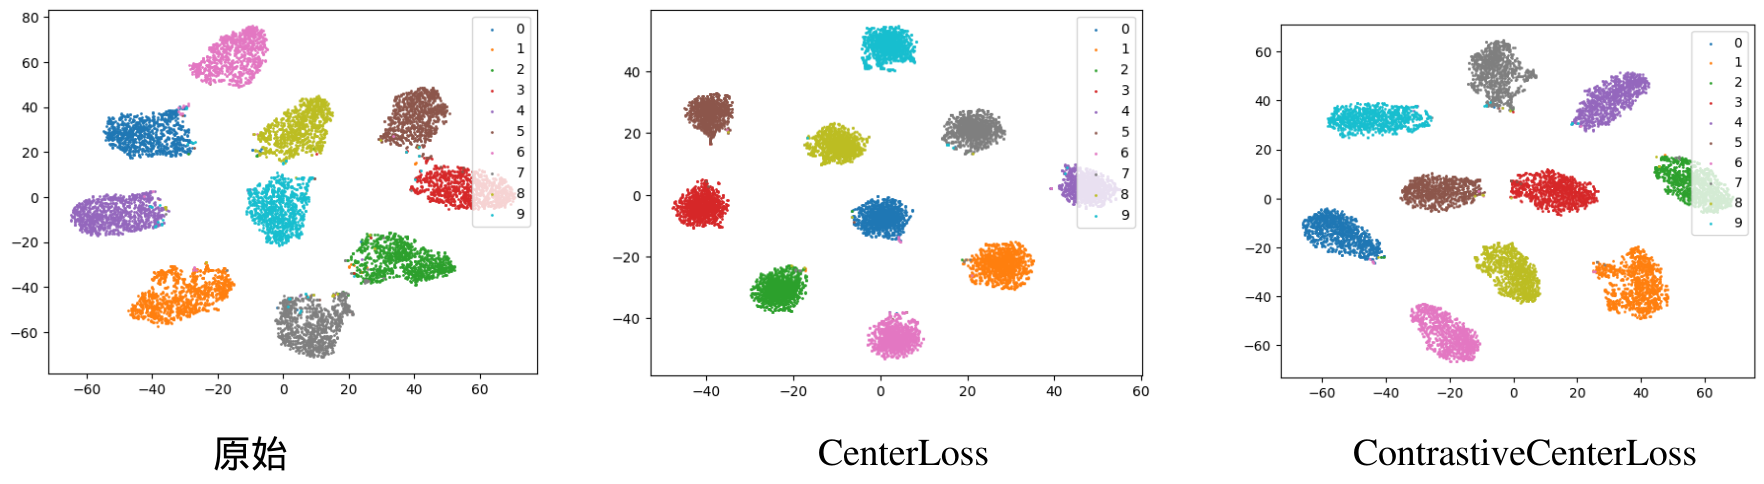
\includegraphics[width=0.8\linewidth]{assets/4-1.png}
    \caption{MNIST特征空间的tsne可视化}
    \label{fig:enter-label}
\end{figure}
\section{辅助损失函数联合训练}
centerloss和contrastive center loss

\begin{figure}[H]
    \centering
    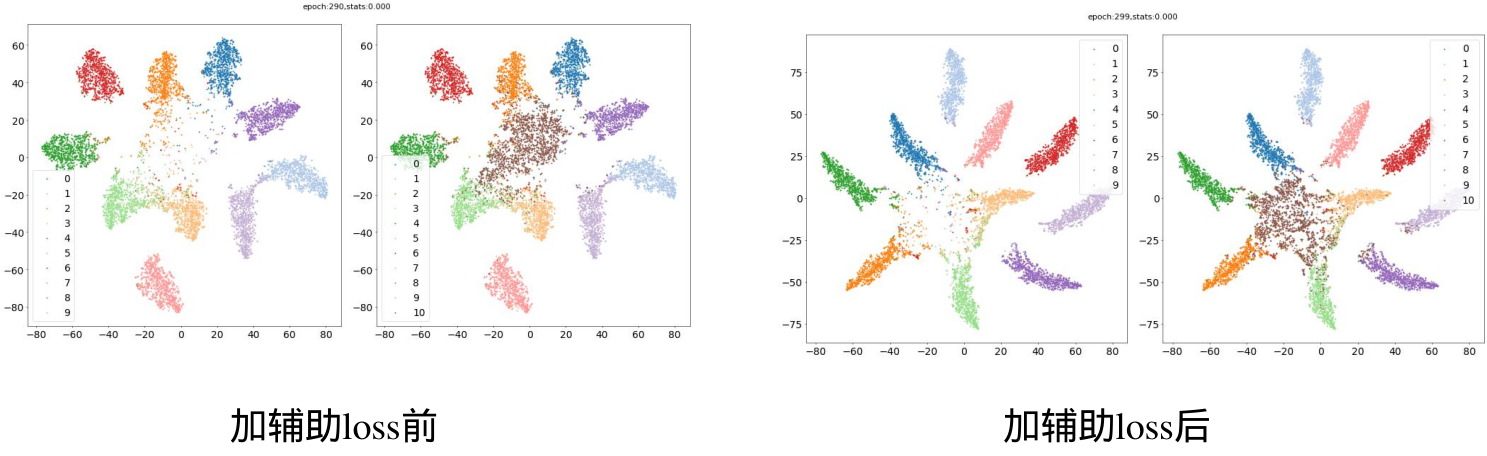
\includegraphics[width=0.8\linewidth]{assets/4-2.png}
    \caption{CIFAR10特征空间的tsne可视化}
    \label{fig:enter-label}
\end{figure}

\section{实验结果与分析}
\subsection{OOD检测任务上评估}
\begin{table}[H]
	\captionsetup{labelformat=empty}
	\centering
	\renewcommand{\arraystretch}{1.2} % 增加行高,提高可读性
	\setlength{\tabcolsep}{8pt} % 调整列间距
	\begin{tabular}{|c|c|c|c|}
		\hline
		\multicolumn{2}{|c|}{\textbf{实验设置}} & \multicolumn{2}{c|}{\textbf{实验结果}} \\ 
		\hline
		\textbf{训练策略} & \textbf{OOD Dataset} & \textbf{ AUROC($\uparrow$)} & \textbf{ AUPRC ($\uparrow$)} \\ 
		\hline
		\multirow{4}{*}{CE loss} 
		& svhn      & 0.9195 & 0.9412 \\ 
		& lsun      & 0.9144 & \textbf{ 0.9317} \\ 
		& cifar100  & 0.8865 & 0.8966 \\ 
		& mnist     & 0.9240 & 0.9426 \\ 
		\hline
		\multirow{4}{*}{CE loss +ContrastiveCenterLoss}
		& svhn      & \textbf{ 0.9332} & \textbf{0.9517} \\ 
		& lsun      & \textbf{ 0.9221} & 0.9270 \\ 
		& cifar100  & \textbf{ 0.8952} & \textbf{0.9065} \\ 
		& mnist     & \textbf{0.9395} & \textbf{0.9579} \\ 
		\hline
	\end{tabular}
	\caption{实验设置:Vgg16+cafar10,D=512,accuracy=0.9438}
\end{table}



\begin{table}[H]
	\captionsetup{labelformat=empty}
	\centering
	\renewcommand{\arraystretch}{1.2} % 增加行高,提高可读性
	\setlength{\tabcolsep}{8pt} % 调整列间距
	\begin{tabular}{|c|c|c|c|}
		\hline
		\multicolumn{2}{|c|}{\textbf{实验设置}} & \multicolumn{2}{c|}{\textbf{实验结果}} \\ 
		\hline
		\textbf{训练策略} & \textbf{OOD Dataset} & \textbf{ AUROC($\uparrow$)} & \textbf{ AUPRC ($\uparrow$)} \\ 
		\hline
		\multirow{4}{*}{CE loss} 
		&	svhn & 0.9260 & 0.9437 \\
		&	lsun &   0.9290 &\textbf{0.9445} \\
		&	cifar100 & 0.9036 & 0.9124 \\
		&	mnist   & 0.9176 & 0.9268 \\
		\hline
		\multirow{4}{*}{CE loss + ContrastiveCenterLoss}
		&	svhn&\textbf{0.9410} & \textbf{ 0.9554}\\
		&	lsun & \textbf{0.9329} & 0.9415 \\
		&	cifar100&  \textbf{0.9115} &\textbf{ 0.9177}\\
		&	mnist  &  \textbf{0.9501} & \textbf{0.9636}\\
		\hline
	\end{tabular}
	\caption{实验设置:ResNet18+cafar10,D=512,accuracy=0.9438}
\end{table}


\begin{table}[H]
	\captionsetup{labelformat=empty}
	\centering
	\renewcommand{\arraystretch}{1.2} % 增加行高,提高可读性
	\setlength{\tabcolsep}{8pt} % 调整列间距
	\begin{tabular}{|c|c|c|c|}
		\hline
		\multicolumn{2}{|c|}{\textbf{实验设置}} & \multicolumn{2}{c|}{\textbf{实验结果}} \\ 
		\hline
		\textbf{训练策略} & \textbf{OOD Dataset} & \textbf{ AUROC($\uparrow$)} & \textbf{ AUPRC ($\uparrow$)} \\ 
		\hline
		\multirow{4}{*}{CE loss} 
		&	svhn & 0.9007 & 0.9008 \\
		&	lsun &   0.9727 & 0.9716 \\
		&	cifar100 & 0.8960 & 0.8966 \\
		&	mnist   & 0.8913 & 0.9123 \\
		\hline
		\multirow{4}{*}{CE loss + ContrastiveCenterLoss}
		&	svhn&\textbf{0.9874} & \textbf{ 0.9910}\\
		&	lsun & \textbf{0.9891} & \textbf{0.9916} \\
		&	cifar100&  \textbf{0.9668} &\textbf{ 0.9704}\\
		&	mnist  &  \textbf{0.9930} & \textbf{0.9939}\\
		\hline
	\end{tabular}
	\caption{实验设置:VIT+cafar10,accuracy=0.9780}
\end{table}

\subsection{对抗样本检测任务上评估}
\section{本章小结}